\RequirePackage{ifpdf}

\documentclass[a4paper,12pt]{article}
\ifpdf
  \usepackage[pdftex]{graphicx}
\else
  \usepackage[dvips]{graphicx}
\fi


\usepackage{epsfig}
\usepackage{rotating}

\usepackage{listings}
\usepackage{booktabs}
\usepackage{fancyhdr}

\usepackage{float}
%\usepackage[config,format=hang,font=small,labelfont=bf,textfont=it,margin=10pt]{caption,subfig}
%\usepackage[format=hang,font=small,labelfont=bf,textfont=it,margin=10pt]{caption,subfig}
%\captionsetup[subfigure]{font=footnotesize}

%\usepackage{attachfile} %should be placed at the end, needed to attach files to a pdf document

%define float placement
\floatplacement{figure}{H}
\floatplacement{table}{H}

\newcommand{\CodeMacro}[2]
{
%\newcommand{\tit}{\textattachfile[color=0 0 0]{code/#1}{#1}}
\newcommand{\tit}{{#1}}
  \lstinputlisting[basicstyle=\footnotesize\ttfamily,
          numbers=left,
          numberstyle=\tiny,
          stepnumber=5,
          numbersep=5pt,
          language={C++},
          frame=tb,
           aboveskip=\bigskipamount,
           belowskip=\bigskipamount,
          captionpos=b,
          label={#2},
          caption={\tit}
]
{code/#1}

}

\newcommand{\CodeCint}[2]
{
%  \renewcommand{\tit}{\textattachfile[color=0 0 0]{code/#1}{#1}}
  \renewcommand{\tit}{{#1}}
  \renewcommand{\thelstnumber}{root [\the\value{lstnumber}]}
  \lstinputlisting[basicstyle=\footnotesize\ttfamily,
          numbers=left,
          numberstyle=\footnotesize,
          stepnumber=1,
          numbersep=5pt,
          language={[GNU]C++},
          frame=tb,
          aboveskip=\bigskipamount,
          belowskip=\bigskipamount,
          xleftmargin=4em,
          framexleftmargin=4em,
          captionpos=b,
          label={#2},
          caption={\tit}
]
{code/#1}

}


\begin{document}

\section*{TPC calibration strategy}
Several different frameworks will be involved in the TPC calibration, including DAQ, HLT, DCS and Offline. Several components inside these frameworks will be involved, among them Detector Algorithms (DA), automatic quality control (AMORE), Offline Calibration Data Base (OCDB).
All calibrations will be based on common calibration classes, which are discussed below. These classes are common for all frameworks. Root files containing these classes are transported between frameworks according to the agreed protocols.

\section{TPC Calibration classes}
\subsection{Calibration tasks:}
\renewcommand{\theenumi}{\arabic{enumi}}
\renewcommand{\labelenumi}{\theenumi.}
\renewcommand{\theenumii}{\alph{enumii}}
\renewcommand{\labelenumii}{\theenumii.}
\begin{enumerate}
 \item Pedestal and noise calibration. 
 \begin{enumerate} 
   \item Pedestal per time bin and pad
   \item Pedestal per pad
 \end{enumerate}
 \item[] Electronic calibration
 \begin{enumerate} 
   \addtocounter{enumii}{2}
   \item Electronics gain calibration (pulser)
   \item Time 0 calibration - Electronic calibration (pulser/data)
   \item Time response function width (pulser/data)
 \end{enumerate}
 \item Gain calibration
 \begin{enumerate} 
   \item Krypton gain calibration
   \item Gain calibration using cosmic (parameterization)
   \item Gain calibration using laser - central electrode plane (pad- by-pad  fluctuation)
   \item Attenuation loss (cosmic)
 \end{enumerate}
 \item Drift velocity calibration. -in relation with 3 c
 \begin{enumerate} 
   \item Laser system - tracks +CE signals (local drift velocity parameterization)
 \end{enumerate}
 \item DCS values in OCDB.
 \begin{enumerate} 
    \item Corrections(p, T)
    \item Goofy (drift velocity, attenuation loss)
    \item Temperature map.
 \end{enumerate}
 \item Space point resolution parameterization and cluster shape parameterization
 \item Space point correction
 \begin{enumerate} 
    \item E distortions (laser) algorithm to be defined.
    \item ExB (B map + laser) algorithm to be defined.
    \item Drift velocity map - parameterization algorithm to be defined.
 \end{enumerate}
 \item Data quality monitoring based on calibration parameters -strongly related with points (1-6)
 \begin{enumerate} 
    \item Noise calibration - Detection of outliers (alarms), FFT spectra for outliers
    \item Electronic gain calibration - Detection  of outliers (alarms)
    \item Time 0 calibration -  	Detection  of outliers (alarms)	
    \item Gain calibration using cosmic - Detection of outliers (alarms)
    \item Space point resolution parameterization and cluster shape parameterization - Pulls for sectors, pad-rows, detection of outliers (alarms)
 \end{enumerate}
 \item Central electrode plane (Unisochronity correction) 
 \item Ion tail characteristics and optimization of filter parameters (laser, cosmic)
 \item Alignment
 \begin{enumerate} 
    \item TPC internal alignment -once per year.
    \item TPC global alignment -every magnetic field change.
 \end{enumerate}
\end{enumerate}



\subsection{Data base entries}

\begin{enumerate}
\item[] \textbf{Existing:}  
  \item Pedestals 
  \item PadNoise
  \item PadTime0 
  \item PadGainFactor      
  \item Parameters - Currently hardwired numbers - drift velocity, sampling frequency
  \item Temperature
  \item Pressure

\item[] \textbf {To be added:}
  \item ALTRO parameters (Frequency, acquisition window, moving average(on/off), zero suppression (on/off), Tail cancellation (on/off)
  \item Drift velocity (Time Stamp),  Attenuation loss  ( TimeStamp)
  \item Alignment
  \item Laser tracks  
\end{enumerate}

\subsection{Calibration entries}

TPC calibration information will be generated by calibration classes running in
DAQ and HLT Detector Algorithms. Each calibration class might generate several
calibration objects, as outlined in figure~\ref{figreference} and
table~\ref{preproctable}. Once all calibration
objects are available, final calibration entries might be calculated based on
the initial entries, as outlined in figure~\ref{figcalib} and table~\ref{ocdbtable}. Calibration objects 
are generated in Detector Algorithms. Collection of calibrations and generation 
of final calibration entries will be performed by the shuttle preprocessor.

\begin{figure}
  \centering\epsfig{figure=images/calib1.eps,width=0.8\linewidth}
  \caption{Preprocessor reference data}
  \label{figreference}
\end{figure}


All calibration entries will be generated by calibration classes. A given
calibration class may generate several calibration objects, see details in the 
table below. The naming convention of the calibration classes is AliTPCCalibXXX,
where XXX gives the calibration task in question (Pedestal, Pulser, CE, Tracks,
LaserTracks etc.) The calibration objects are correspondingly named tpccalibXXX.


\section{Calibration procedure}
All calibrations are calculated based on measured data using the standard TPC
readout chain. Pedestals and noise are generated using special "black" triggers,
where a signal is generated in all readout pads. Such triggers are collected in
special runs, identified by RunType $==$ PEDESTAL. The pedestal/noise values are not expected to change during a physics run. The maximum frequency of pedestal runs is one such run before each physics run, once experience on the stability of the pedestal/noise measurements is obtained, it may be decided to reduce this frequency. 

Pulser triggers are used to measure the performance of the readout electronics.
A special pulse is given to the gating grid, causing readout from all pads. The
performance of the electronics is not expected to change during the physics run,
and pulser triggers are also taken in special runs, identified by RunType $==$ 
PULSER.

The drift velocity of the TPC is monitored by measuring signals generated by
laser pulses at the Central Electrode (CE). The drift velocity depends on
environmental parameters (temperature, pressure etc.) and may change during
the physics run. The laser triggers are therefore produced at fixed intervals
during the physics run, identified as a LASER\_EVENT in the trigger mask. 

\begin{table}
 \caption{Preprocessor reference data}
 \begin{sideways}
 \label{preproctable} 
 \begin{tabular}{|l|l|l|l|l|l|} \hline
  Calibration class & System & \multicolumn{2}{|l|}{Reference data} &
  \multicolumn{2}{|l|}{OCDB entry} \\ \cline{3-6}
  AliTPCCalibXXX & & name & size & names & size  \\ \hline 
  Pedestal & DAQ, HLT & tpcCalibPedestal & 107.5 MB & pedestalMean & 2.2 MB \\
           &          &                  &          & pedestalRMS & 2.2 MB 
  \\ \hline 
  Pulser  &  DAQ   & tpcCalibPulser      & 538.2 MB & pulserTmean & 2.2 MB \\
          &        &                     &          & pulserTrms  & 2.2 MB \\
	  &        &                     &          & pulserQmean & 2.2 MB
  \\ \hline 
  CE      &  DAQ   & tpcCalibCE          & 538.2 MB & CETmean     & 2.2 MB \\
          &        &                     &          & CETrms      & 2.2 MB \\
	  &        &                     &          & CEQmean     & 2.2 MB
  \\ \hline 
  Tracks  & HLT, Offline & tpcCalibTracks & ??      & ClusterParam & small \\
          &              & tpcCalibTracksGain & ??  & PadGainFactor &      \\
	  &              &                    &     & ClusterParam  &      \\
	  &              & tpcCalibTracksAlign & ?? & TPCAlignment  &    \\
	  \hline
  LaserTracks & HLT, Offline & tpcCalibLaserTracks & ?? & TPCAlignment & small
  \\ \hline 
  PIDV0   & Offline & tpcCalibPIDV0      & ??       & ??           & small
  \\ \hline 
  DCS     &         &                &        & Temperature & 200 kB \\
          &         &                &        & Pressure    & 1 kB \\
	  &         &                &        & GasComposition & 1 kB \\
	  &         &                &        & Voltages    &       \\ \hline
  \end{tabular}
 \end{sideways}
\end{table}


\subsection{OCDB Calibration entries}
Based on the calibration objects described above, final OCDB calibration entries
will be generated by the TPC Shuttle preprocessor. The OCDB calibration entries
will be used to correct TPC raw data for offline processing.
 
The Pedestal and PadNoise entries will be regnerated each calibration run, based
on data from the AliTPCCalibPedestal calibration object. The PadTime0 entry will
extract data both from AliTPCCalibPulser and AliTPCCalibCE. The combined entry
will be regenerated during physics run (AliTPCCalibCE), and will use information
from the previous pulser run, as available in the OCDB. 

The PadGainFactor calibration will require several iterations, and will be
carried out by a standalone calibration procedure, not being part of the
DA/Shuttle framework. The resulting calibration entry will be valid for a long
time frame, and the produced data base entry will be available for the
quasi-online reconstruction.

\begin{table}
 \caption{Final OCDB entries}
 \label{ocdbtable} 
 \begin{tabular}{|l|l|l|l|} \hline
 OCDB entry & size & \multicolumn{2}{|l|}{Reference data} \\ \cline{3-4}
            &      & name & size \\ \hline
 Pedestal & 2.2 MB & PedestalMean (AliTPCCalPad) & 2.2 MB \\ \hline
 PadNoise & 2.2 MB & PedestalRMS  (AliTPCCalPad) & 2.2 MB \\ \hline
 PadTime0 & 2.2 MB & PulserTmean  (AliTPCCalPad) & 2.2 MB \\ 
          &        & CETmean      (AliTPCCalPad) & 2.2 MB \\ \hline
 PadGainFactor &   & PulserQmean  (AliTPCCalPad) & 2.2 MB \\
          &        & CEQmean      (AliTPCCalPad) & 2.2 MB \\ 
	  &        & TracksGain   (AliTPCCalPad) & 2.2 MB \\ \hline
 DriftVelocity & ?? & CETmean (AliTPCCalPad or TObjArray) &  \\ \hline 
 Attenuation   & ?? &                                     & \\ \hline
 Parameters    &    &                                     & \\ \hline
 Temperature   & 200 kB & DCS (AliSplineFit)              & \\ \hline
 GasComposition &       & DCS (AliSplineFit)              & \\ \hline
 HighVoltage   &        & DCS (AliSplineFit)              & \\ \hline
 \end{tabular}
\end{table}  

\begin{figure}
  \centering\epsfig{figure=images/calib2.eps,width=\linewidth}
  \caption{Final calibration data}
  \label{figcalib}
\end{figure}


\section{Calibration in the AMORE framework}
\subsection{General overview}

Calibration will run in DAQ and HLT Detector Algorithms. Each of these will
produce a series of calibration classes. The calibration classes will contain
functionality to produce histograms, trees and time-dependent graphs to be fed
into AMORE. In general histograms will be used for the automatic monitoring,
and trees will provide input for interactive expert monitoring. Both histograms 
and trees will be wrapped in monitoring objects\footnote{Encapsulating calibration
objects originating from the HLT DAs generates problematic dependencies in the 
current setup. It will be necessary to find a scheme to communicate the relevant 
objects with a minimum of induced overhead, for instance by including 
lightweight classes to generate these objects in AliRoot STEER.} 
before being submitted to AMORE. 

The AMORE framework will take care of collecting subtrees from various DAs to 
produce a full tree for the expert monitoring. It will be decided later whether 
this collection will take place continuosly or only when triggered by a request 
from the Expert monitor.  Reference trees and the most recent tree will be 
available at any time, but previous trees will normally not be stored. It might 
be of interest to allow AMORE alarms to trigger storage of the current tree to 
some intermediate storage. The data flow to AMORE is illustrated in the
figure~\ref{amorefigure}.

\subsection{Histograms}
We plan to generate 7 sets of histograms, for pedestals, noise, gain, t0, width,
gain with Central Electrode and drift velocity from Central Electrode signal.  
Each of these signals will be histogrammed sector by sector (each sector is 
divided in two read-out chambers, so altogether this makes 72 2-dimensional 
histograms). For each signal there will be three set of histograms: pad-by-pad 
histograms (2-dim), 1-dim histograms of values (mean value, median, LTM, 
fraction of outliers) and 2-dim profile histograms (mean value per pad row), 
altogether 2*72*7 2-dimensional histograms and 4*72*7 1-dimensional histograms. 
These histograms should be automatically monitored/compared to reference 
histograms, and "status" or "quality" histograms could be generated based on 
these comparisons.

We would also like to monitor the phase of each readout partition, i.e. one 
histogram per event with 216 bins corresponding to the readout partitions. 
Other variables to be monitored are the drift velocity and gain parameters as 
function of time. Here we will have 
72 (chambers)x3(fit parameters)x2(drift, gain) graphs value versus time.  

All histograms can be generated from TPC calibration classes (AliTPCCalPad).
To get Median, LTM , Mean, RMS, outliers list, we have functionality inside TPC 
calibration classes. Selected histograms will be accumulated as histograms of 
differences with respect to reference trees.

In addition to this we will have histograms based on cluster and track 
information. These histograms will be generated by the HLT, and submitted to 
DAQ through the HLT/DAQ interface (HLT appears as a "subdetector" in DAQ).
 
\subsection{Expert monitor}
The expert monitor will read full trees to be collected in AMORE, based on 
subtrees generated by the calibration classes obtained from DAQ and HLT DAs. 
The expert monitor will give interactive access to the full calibration 
information to allow for efficient detector problem resolution.

\subsection{Histogram sizes}
The size of 2D histograms is on the level of 2 MBy per TPC side. 7x2 MBy ~ 14 MBy.
The size of other histograms is negligible in comparison with this one. Total 
size will be around ~ 20MBy. If we want to compare results with reference 
histograms we should multiply it by 2 ~ 40 MBy.
  
\subsection{Refresh frequency}
Entries for the calibration histograms should be generated whenever a laser 
trigger or a calibration pulse trigger occurs. The frequency of these triggers 
have not yet been decided, but they will not exceed 1 Hz and 0.01 Hz 
respectively. Depending on the signal, 10-100 such triggers are necessary to 
obtain a reliable histogram which could be compared to reference histograms. 
Comparison should happen continuously once these numbers of calibration 
triggers are reached. This would lead to the following maximum repetition 
times: gain, t0, width:   0.001Hz. 
Pedestal and noise information will be collected from special triggers taken at 
the beginning and the end of each run. At the periods these triggers are 
activated, they will occur with a frequency of 0.1 Hz.
Comparison to reference histograms will be made at each end-of-run.

The parameters drift velocity and gain will be calculated from special laser 
triggers, with a frequency of about 0.01 Hz. These calibrations will be handled 
by HLT. The drift velocity calibration might be updated for each such trigger, 
whereas the gain calibration will be updated when about 1000 tracks are recorded 
(which will correspond to several times per run).

\subsection{Time dependence}
Graphs will be generated containing amplitude vs. time, drift velocity vs. time.
These will be based on pedestal/noise measurements done at the end of each run.
 We will also record baseline and noise vs. time.

\subsection{Global events}
We need access to global events to monitor drift velocity and gain using CE. 
We assume that the signal coming from the CE and readout by the different 
readout partitions (RCUs) is synchronous with either the sampling clock or the 
40 Mhz clock. In the latter case, we need to know the phase of the trigger with 
respect to the sampling clock. Other calibrations can be done patch by patch, 
i.e. on the LDCs. Calibration tasks run on HLT will need access to ITS and TRD 
information, but this communication will be handled internally in the HLT system.

\subsection{Event reconstruction}
All calibration tasks that need access to reconstruction will be performed by
the HLT, and use HLT reconstruction.

\subsection{External access} 
We need access to reference histograms and trees. We will also need access to
temperature and pressure graphs from DCS. These graphs will be accumulated using
HLT, and will be forwarded to AMORE as part of the HLT calibration classes.

\subsection{Critical errors}
Discovery of wrong phase, intensity of laser below fixed limit, missing 
patches/sectors would severely affect the quality of the data, and should 
trigger alarms.



\begin{figure}
  \centering\epsfig{figure=images/amore.eps,width=\linewidth}
  \caption{AMORE calibration flow for the TPC}
  \label{amorefigure}
\end{figure}


\section{Quality assurance}

Data quality monitoring is based on monitoring of statistical properties of the
data. A big fraction of the properties to be monitored are extracted during the
calibration procedure.  The QA procedure will evolve in time together with the 
further development and tuning of the calibration algorithm.  

We consider two modes of the QA algorithms:

\begin{itemize}
 \item Tuning phase  (mainly expert mode)
 \item Standard operation 
\end{itemize}

The expert mode of QA will be particularly important during the commissioning phase 
of ALICE. The  main additional functionality implemented in the expert mode is 
the possibility to generate statistical graphs using correlation with other 
variables and make custom selections. These will help us to better understand 
the processes in the detector, and make the transition to the standard operational
mode faster.

   

\subsection{Tuning phase}

Detect the problems.
Define, what is the problem

What do we expect? 
Defined in the TPC TDR and in the PPR on the basis of simulation
How far we are from the expectation?
Modify expectation.

Until which point the information from the detector is reasonable?
Define the limits of working conditions.
Up to which point the physics performance will not be influenced.
What impact the observed imperfection could make on physics performance.

In the following we put focus on these topics.







\subsubsection{Quality  assurance  - pedestal and noise}

According to the TPC TDR the electronic noise of Alice TPC was designed to be on 
the level of 1000 e, which correspond to 1 ADC channel (TPC TDR). The most probable
signal to noise ratio was about 20 in inner chambers and $\sim$ 30 in the outer
chambers. In such a set-up the space resolution and the dEdx  resolution is 
determined by other stochastic processes like diffusion and angular effects. 
E.g for space resolution the diffusion component is of the order of $\sim$ 0.7 mm 
while the noise component $\sim$ 0.2 mm. The spatial resolution can be affected by 
lowering the gain or increasing the noise level. E.g increasing the noise by 
factor of 3,  the mean space resolution will be worsened by a factor $\sim$ 15\%. 

The requirements for pedestal knowledge are determined mainly by dEdx 
measurement. The relative dEdx resolution in the Alice TPC is on the level of 5\%. 
In order to know the pedestal on the level of 1 \% of the 
most probable signal (~ 10-20 ADC channel), the required precision and stability
of the pedestal should be on level of 0.1 ADC. The pedestal and noise will be 
measured before each physics run. The experience from TPC tests in 2006 
indicates that such a frequency is sufficient.

\begin{table}
\begin{tabular}{|l|r|r|r|} \hline
  \multicolumn{1}{|c|}{noise(ADC)} & \multicolumn{1}{|c|}{2} &
  \multicolumn{1}{|c|}{3}& \multicolumn{1}{|c|}{4} \\ \hline
space resolution worsening factor &  1.05 & 1.15 & 1.3 \\ \hline
\end{tabular}
\end{table}
         
The TPC test in 2006 showed that the mean observed  noise in the TPC is even 
better than the original requirement ($\sim$ 0.7 ADC in IROC).  Problems were encountered 
at the edges of the chambers, which are more sensitive to noise induction. 
As a consequence the noise can be much higher at the edges and the noise 
distribution can be highly non-Gaussian.  Therefore, some robust statistic 
should be used for its estimation.

Input data:
\begin{itemize}
 \item TPC raw data without zero suppression preprocessed by the calibration 
      algorithm AliTPCCalibPedestal.
 \item AliTPCCalibPedestal produce the noise and pedestal maps.
 \item The noise maps (AliTPCCalPad)  - current and reference.
 \item The pedestal maps (AliTPCCalPad) - current and reference.
\end{itemize}

Histograms and graphs to be monitored:
\begin{itemize}
 \item Noise and pedestal distribution for each sector.
 \item Cumulative noise distribution.
 \item Distribution of the differences between pedestal and noise from
      reference runs.
 \item The median of the noise distribution as a function of sector
 \item The median of the noise distribution as a function of time
\end{itemize}

All these can be generated by AliTPCCalPad. Moreover in the expert mode using
the trees, selections can be be made applying user defined cuts  .

Observables to be checked:
\begin{itemize}
 \item Mean and median of the noise distribution - Alarms on median
 \item The fraction - p0 of  "non usable" channels - The noise bigger
       than a threshold th0 (e.g 4 ADC)  
 \item The fraction - p1 of "suspicious" channels - The noise bigger than
       a threshold th1 (e.g 2 ADC)
\end{itemize}

\subsubsection{Quality  assurance  - not responding channels}

The Alice TPC consists of 159 pad rows.  Signals from these pad rows are used in
order to extract the properties of the tracks. The resolution of the variables
are scaling as square root of the number of used measurement points.  By simple
scaling, the absence of 10 \% of the channels lead to 5 \% deterioration of the 
performance.
  
There are following reasons:
\begin{itemize}
 \item Electronic problems. (e.g missing contacts)
 \item Single event upset. 
 \item Data corruption during data readout.
\end{itemize}

The fraction and maps due to the latter two reasons can change on a time scale
smaller than one run.

Otherwise we consider changes on the run level. The special pulser will be
used to generate the dead map channel maps.  

To eliminate or reduce the fraction of not responding channels due to data
corruption, the decoding algorithm should be made robust enough, and minimal 
amount of channels (digits) should be skipped in case of the detection of data 
corruption.  

Missing channels due to the single event upset should be on negligible level 
(much below  \% level)

The results for the TPC test 2006 indicates the amount of the dead - not 
responding - channels on the level below 1 per mile.  

To produce the dead channel map the output of the pulser calibration can (will)
be used (AliTPCCalibPulser). 

Input data:
\begin{itemize}
 \item Raw data sets with pulser $==>$ AliTPCCalibPulser
 \item The amplitude maps (AliTPCCalPads)
 \item The time maps (AliTPCCalPads) 
\end{itemize}

The typical dispersion of the electronics gain is on the percent level. Results
from the TPC test in 2006 show some fraction of the outliers with significantly
higher response. Such outliers are grouped close to the pulser connectors.  
There were no observation of outliers in other directions, except of the pads 
not responding at all.

Histograms and graphs to be monitored:
\begin{itemize}
 \item The amplitude distribution for each chamber and each pad geometry.
 \item Graphs of the median of the amplitude distribution.
\end{itemize}

Observables to be checked:
\begin{itemize}
 \item The fraction of the pads with signal below p1 ratio of the median 
      (for given pad type). 
\end{itemize} 


%---------------------------------------------------------------------------------------------------------
%-
%-                                                Calibration class description
%-
%----------------------------------------------------------------------------------------------------------
\section{Description of the calibration classes}
In this chapter the working principles of the three calibration classes ``AliTPCCalibPedestal'', ``AliTPCCalibPulser'' and ``AliTPCCalibCE'' will be explained in detail. After an introduction about the commonalities of the classes (interface, work flow), each algorithm will be on its own.

\subsection{Common introduction}
The general idea of the calibration classes is to process and analyse raw data. The algorithms are supposed to run in different environments, such as in the offline reconstrution, the high level trigger or in the data acquisition system.
% \subsection{Event processing}
To guarantee flexibility in the data processing, several methods are available calling each other in a hirachical order. For the decoding of the raw data two different algorithms are available which led to two branches of processing functions.
The relavent functions are called {\bf ProcessEvent[Fast]} taking as an input either the DATE  {\bf eventHeaderStruct} an {\bf AliRawReader} object or an {\bf AliTPCRawStream[Fast]} object.
The function which does the actual processing of the data is called {\bf Upate} and takes as arguments the sector, pad row, pad, time bin and adc signal. All this is summariesed in fig.\ \ref{fig:calib.process}.

\begin{figure}
  \centering
  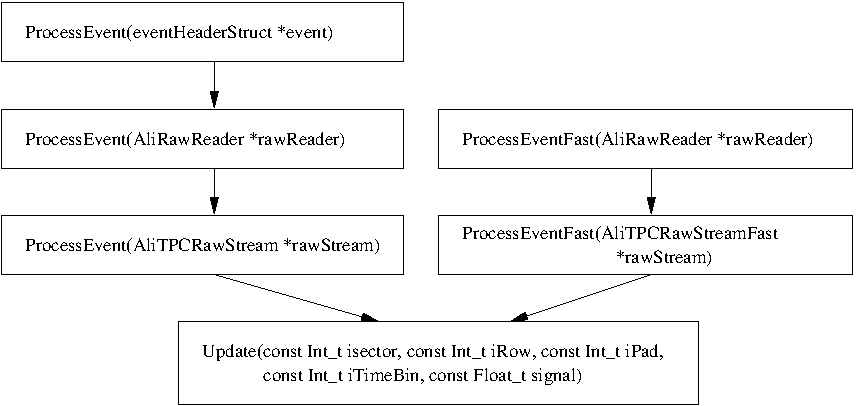
\includegraphics[width=0.9\linewidth]{images/ProcessFunctions}
  \caption{Hirachy of the event processing functions of the calibration algorithms.}
  \label{fig:calib.process}
\end{figure}

The calibration data is stored in {\em reference histograms}, filled in the {\bf Update} function, functions called inside, and the {\bf EndEvent} function. For each readout chamber and calibration variable {\it XXX} one reference histogram is created. These are two dimensional having on the y-axis the channel number within the ROC and on the x-axis the distribution of the calibration variable. Setters exist to adjust the range and number of bins. An example of a reference histogram can be found in fig.\ \ref{app:calib.refhist}.

Inside the calibration class the reference histograms are stored in {\em TObjArrays}, one for each variable keeping the 72 histograms for the ROCs. The arrays are called {\bf fHisto{\it XXX}Array} and can be retrieved with the getter function {\bf GetHisto{\it XXX}}(Int\_t sector, Bool\_t force=kFALSE). To allocate memory only if needed, the histograms are created the first time the getter is called and the force flag is set to kTRUE.

\begin{figure}
  \centering
  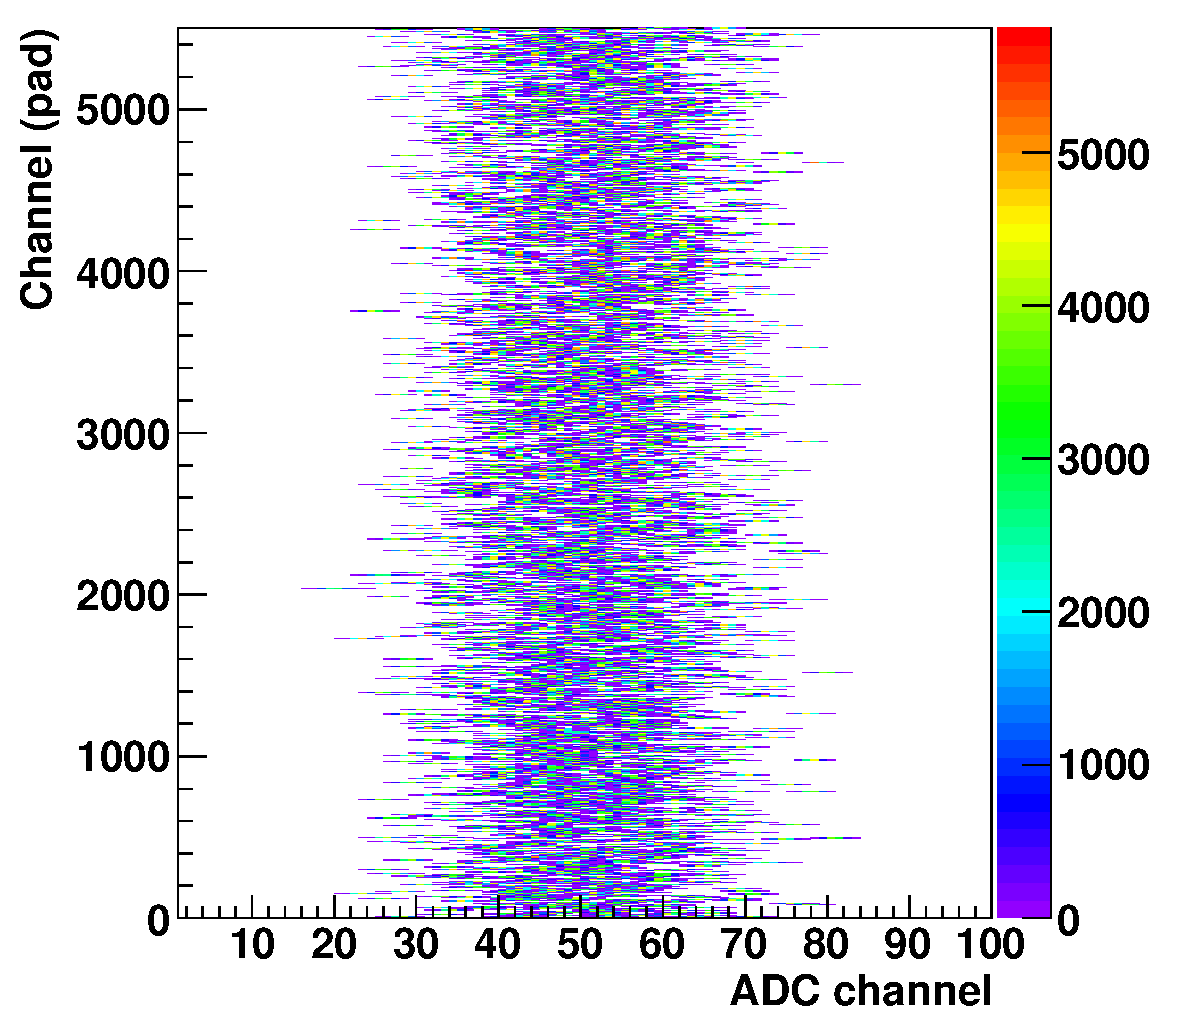
\includegraphics[width=7.3cm]{images/RefHist}
  \caption{Example of a reference histogram. Displayed are the electronic baseline distributions for all pads of one IROC.}
  \label{fig:calib.refhist}
\end{figure}

For the Pulser and CE calibration after each event the {\bf EndEvent function} has to called, doing some post processing, the filling of a part of the reference histograms and calculation of data stored event by event (see description below).

After the desired statistics has been accumulated the actual calibration values pad by pad are calculated by calling the {\bf Analyse} function. To store the data a special class {\bf AliTPCCalROC} is used keeping all values for one readout chamber. As in case of the reference histograms, the AliTPCCalROC objects are only created upon request, by using the getter function {\bf GetCalRoc{\it XXX}}(Int\_t sector, Bool\_t force=kFALSE) with the force flag set to kTRUE. The objects are also stored in {\em TObjArrays} which are called {\bf fCalRocArray{\it XXX}}. A pointer the complete arrays is provided by the {\bf GetCalPad{\it XXX}}() functions.

To save the calibration data the function {\bf DumpToFile} is available, taking as arguments the filename and optional a directory name to which it should be stored in the file and if the file should be updated instead of overwritten.

The process flow described above is summarised in fig.\ \ref{fig:calib.calibflow}

\begin{figure}
  \centering
  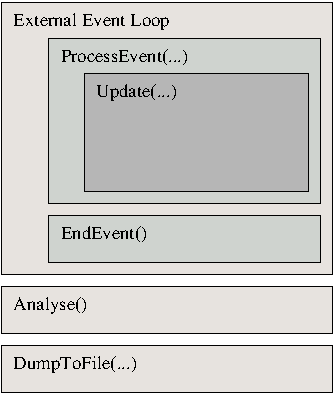
\includegraphics[width=7cm]{images/ProcessFlow}
  \caption{Process flow of the calibration algorithms.}
  \label{fig:calib.calibflow}
\end{figure}

%################################################################################
\subsection{Pedestal calibration class}
\subsubsection{Signal filling {\small [Update(\dots)]}}
The {\bf Update} function fills the reference histograms with the ADC values of all time bins in the selected range (fFirstTimeBin, fLastTimeBin) with standard values (60, 1000). The range can be specified by the setter function {\bf SetRangeTime}(Int\_t tMin, Int\_t tMax).
If requested by {\bf SetTimeAnalysis}(Bool\_t time = kTRUE), pedestal values for each time bin will be calculated. This information can be used to fill the pattern memory of the ALTRO in order to perform a timebin by timebin baseline subsection.

\subsubsection{Calibration value calculation {\small [Analyse()]}}
Calling the {\bf Analyse}() routine calculates the pedestal and noise values for each channel by fitting a gaus function on the distribution. In addition a second approach is used calculating the mean and corresponding RMS. If desired a truncation range can be set using the {\bf SetAnalysisTruncationRange}(Float\_t down, Float\_t up) function, where down and up mark the range as a fraction of the data: e.g. (0.05,0.9) would exclude the lower 5\% and upper 10\%.

\subsubsection{Stored calibration values}
The available calibration values calculated in the pedestal calibration class, a description as well as the corresponding getter functions are summariesed in table\ \ref{app:tab.pedestal}

\begin{table}[H]
  \footnotesize
  \centering
  \begin{tabular}{l|p{3.2cm}|l|l}
  \hline
  {\bf Cal. value} & {\bf description} & {\bf getter} {\scriptsize (AliTPCCalROC*)} & {\bf getter} {\scriptsize (TObjArray*)}\\
  \hline
  \hline
  Pedestal & pedestal value\newline {\footnotesize (mean of a gaus fit)}       & GetCalRocPedestal(sector) & GetCalPadPedestal() \\
  Sigma    & noise value\newline {\footnotesize (sigma of a gaus fit)}         & GetCalRocSigma(sector)    & GetCalPadSigma() \\
  Mean     & pedestal value\newline {\footnotesize (mean of the distribution)} & GetCalRocMean(sector)     & GetCalPadMean() \\
  RMS      & noise value\newline {\footnotesize (rms of the distribution)}     & GetCalRocRMS(sector)      & GetCalPadRMS() \\
  \hline
  \end{tabular}
  \caption{Calibration values}
  \label{app:tab.pedestal}
\end{table}

%################################################################################
\subsection{Pulser calibration class} \label{app:calib.pulser}
\subsubsection{Signal filling {\small [Update(\dots)]}} \label{app:calib.pulser.updated}
In the {\bf Upate}(\dots) function of the Pulser Calibration class an array (fPadSignal) is filled with the ADC signal information for each timebin of the currently processed channel (pad). In addition the maximum ADC value and corresponding timebin is stored (fMaxPadSignal, fMaxTimeBin). Only the selected time range (fFirstTimeBin, fLastTimeBin) is taken into account. The range can be set by calling {\bf SetRangeTime}(Int\_t firstTimeBin, Int\_t lastTimeBin). Before proceeding with the next channel, the {\bf ProcessPad}() function is called, which analyses the information currently stored in fPadSignal.

\subsubsection{Channel information processing {\small [ProcessPad()]}}
As a first step the pedestal and noise values for the current pad are queried ({\bf FindPedestal}()). Therefore either previouly measured data can be used ({\bf SetPedestalDatabase}(AliTPCCalPad *pedestalTPC, AliTPCCalPad *padNoiseTPC)) or if not set the pedestal and noise will be calculated. This is done by calculating the truncated mean and RMS within a range of $\pm 10$\,ADC channels around the median of the signal distribution stored in fPadSignal.

In the second step the properties of the pulser signal are calculated ({\bf FindPulserSignal}(\dots)). For the analysis it is assumed that there is only one signal which spreads over a range of minus two to plus seven timebins around fMaxTimeBin. After the pedestal substraction the signal sum, mean and RMS are calculated in this range. If the signal sum is below a threshold of 8 times the pad noise (minimum noise set to 1 ADC count), all values are set to zero.

As a third step the reference histograms for the charge (signal sum) and signal width information are filled. The time position (signal mean) is stored in an array for later processing (see below).

\subsubsection{Event information processing {\small [EndEvent()]}}
The {\bf EndEvent}() function loops over all readout chambers and filles the time information into the reference histograms. Stored is the deviation from the mean of the time signals in the currently processed ROC.

\subsubsection{Calibration value calculation {\small [Analyse()]}}
In the {\bf Analyse}() function the final calibration values are calculated as the mean of the distributions stored in the reference histograms. The information is finally stored in AliTPCCalROC objects.

\subsubsection{Stored calibration values}
The available calibration values calculated in the pulser calibration class, a description as well as the corresponding getter functions are summariesed in table\ \ref{app:tab.pulser}

\begin{table}[H]
  \footnotesize
  \centering
  \begin{tabular}{l|p{3.2cm}|l|l}
  \hline
{\bf Calib. value} & {\bf description} & {\bf getter} {\scriptsize (AliTPCCalROC*)} & {\bf getter} {\scriptsize (TObjArray*)}\\
  \hline
  \hline
  T0  & time position {\footnotesize (relative to chamber mean)} & GetCalRocT0(sector) & GetCalPadT0() \\
  \hline
  Q   & signal sum          & GetCalRocQ(sector)    & GetCalPadQ() \\
  \hline
  RMS & signal width        & GetCalRocRMS(sector)  & GetCalPadRMS() \\
  \hline
  \end{tabular}
  \caption{Calibration values in the pulser calibration class}
  \label{app:tab.pulser}
\end{table}


\subsection{Central electrode signal calibration class}
\subsubsection{Signal filling {\small [Update(\dots)]}}
Before calling either the {\bf ProcessEvent}(\dots) or the {\bf Update}(\dots) function, {\bf SetEventInfo}(Double\_t runNumber, Double\_t timestamp, Double\_t eventId) should be called for each event to be able to display some of the stored calibration values as one a function of on of these information. The {\bf Update}(\dots) function itself is exactly the same as described above in the Calibration Pulser section (\ref{app:calib.pulser.updated}).

\subsubsection{Channel information processing {\small [ProcessPad()]}}
The first step is getting the pedestal and noise values (see \ref{app:calib.pulser.updated}).

In the second step local maxima are searched in the pad signal ({\bf FindLocalMaxima}(\dots).  For each chamber a histogram is filled with this information. To be accepted as a local maximum the signal has to be five times larger than the pad noise and needs 2(3) preceding (succeeding) timebins with a falling signal height. Maxima are expected to arise from the laser rays, photoelectrons from the central electrode, but also periodic post peaks following the CE signal have been observed. The largest fraction however arising from the CE. In the {\bf EndEvent}() function for each ROC the time position of the maximum of the local maxima distribution will be calculated, identified with the time position of the central electrode and stored event by event in an array ({\it fTMeanArrayEvent}).

If no event has been processed yet in this run no further processing on the pad signal will be done. The reason is that no position information of the central electrode signal is available at that point.

The third step is the analysis of the central electrode signal ({\bf FindCESignal}(\dots)). To decide which of the local maxima found before represents the CE signal, the distance to the identified position of the previous event (see end of second step) is calculated. The maximum with the smallest distance is used. Signal sum, mean and RMS are calculated in a range of -4 to +7 timebins around the maximum. If the signal sum is smaller than eight times the pad noise, all values will be set to zero.

The fourth step filling of the signal sum and width histograms, as well as filling a temporary array with the time (signal mean) information.

\subsubsection{Event information processing {\small [EndEvent()]}}
In the beginning of the function the mean drift time for each readout side is calculated.

Next it is looped over all sectors for which information are available. If the local maxima distribution histogram has less entries than 2/3 of the number of channels of the ROC, it will be skipped. This is the reason if the calibration algorithm is run on data which has no laser events.

As already described above the maximum position of the local maxima distribution is calculated. For this purpose the truncated mean within a range of $\pm4$ timebins around the median of the distribution is used.

To monitor the stability of the laser, the mean charge (signal sum) is calculated for each ROC and stored event by event.

In a loop over all channels the time reference histograms are filled with the difference of the pad time  signal to the mean arrival time of the corresponding readout side, calculated above. This approach is used to accumulate statistics over a long time range in which the drift velocity might change. Non time dependend and time dependend effects are such hoped to be decoupled to a large extent. In addition a temporary AliTPCCalROC object is filled with the time inforation.

The AliTPCCalROC object is used to perform a linear as well as parabolic 2D fit to the data. This information is stored event by event and can be used to study non uniform changes in the drift velocity.

\subsubsection{Calibration value calculation {\small [Analyse()]}}
In the {\bf Analyse}() function the final calibration values are calculated as the mean of the distributions stored in the reference histograms. The information is finally stored in AliTPCCalROC objects.

\subsubsection{Stored calibration values}
The available calibration values calculated in the pulser calibration class, a description as well as the corresponding getter functions are summariesed in table\ \ref{app:tab.ce}

\begin{table}[H]
  \centering
  \footnotesize
  \begin{tabular}{l|p{3.2cm}|l|l}
  \hline
{\bf Calib. value} & {\bf description} & {\bf getter} {\scriptsize (AliTPCCalROC*)} & {\bf getter} {\scriptsize (TObjArray*)}\\
  \hline
  \hline
  T0  & time position {\footnotesize (relative to the readout side)} & GetCalRocT0(sector) & GetCalPadT0() \\
  \hline
  Q   & signal sum          & GetCalRocQ(sector)    & GetCalPadQ() \\
  \hline
  RMS & signal width        & GetCalRocRMS(sector)  & GetCalPadRMS() \\
  \hline
  \end{tabular}
  \caption{Calibration values in the central electrode calibration class}
  \label{app:tab.ce}
\end{table}

As described above additional data is stored event by event for each chamber. Table \ref{app:tab.ceebye} summarieses the information, gives a short description and shows the getter function.
\begin{table}[H]
  \centering
  \footnotesize
  \begin{tabular}{p{4cm}|l|p{4cm}}
  \hline
{\bf type of information} & {\bf getter } & {\bf description} \\
\hline\hline
results of a plane fit  & GetParamArrayPol1(sector) & {\small returns a TObjArray of TVectorD objects, one entry per event}\\
\hline
results of 2D parabolic fit  & GetParamArrayPol2(sector) & {\small returns a TObjArray of TVectorD objects, one entry per event}\\
\hline
mean arrival time & GetTMeanEvents(sector) & returns an array of floats (TVectorF), one entry per event\\
\hline
mean signal sum & GetQMeanEvents(sector) & returns an array of floats (TVectorF), one entry per event\\
\hline
  \end{tabular}
  \caption{Event by event information stored for each chamber in the central electrode calibration class}
  \label{app:tab.ceebye}
\end{table}


\subsection{Using the Calibration Classes} \label{app:code.calib}
% \subsection{Data processing}
Listing \ref{app:code.fillcalib} shows an example how to loop over one root raw data file to fill one of the calibration classes for either Pedestal and Noise calibration, analysing data taken with the Calibration Pulser or retrieving information from the Central Electrode signal acquired from events using the TPC laser system.

The code shows a ROOT macro that is supposed to be executed from the commandline prompt in the ALICE offline analysis framework AliRoot. In the example {\em XXX} has to be replaced bei one of {\em Pedestal}, {\em Pulser} or {\em CE}.

Examples of how to load the macro and execute it is shown in listing \ref{app:code.pedestal} for the case of a pedestal run and \ref{app:code.pulserCE} in case of a pulser or laser run. The listings also demonstrate the possibility of displaying the stored calibration data using the AliTPCCalPad class. For more information see the documentation in the class code.

\CodeMacro{fillCalibObject.C}{app:code.fillcalib}
\CodeCint{commandsPedestal.cint}{app:code.pedestal}
\CodeCint{commandsPulserCE.cint}{app:code.pulserCE}


\section{HTML Documentation}


\begin{description}
 \item[AliTPCCalibPedestal]\mbox{}\\ 
  http://aliceinfo.cern.ch/static/aliroot-new/html/roothtml/AliTPCCalibPedestal.html
 \item[AliTPCCalibPulser] \mbox{}\\
  http://aliceinfo.cern.ch/static/aliroot-new/html/roothtml/AliTPCCalibPulser.html
 \item[AliTPCCalibCE] \mbox{}\\
  http://aliceinfo.cern.ch/static/aliroot-new/html/roothtml/AliTPCCalibCE.html
\end{description}


\end{document}
